We now investigate the CFL condition of the Lax-Friedrichs program from our previous report. Here, we show the results of the Lax-Friedrich for various values of $\Delta t/\Delta x$, given epsilon=0.1, alpha=$\Delta x/\Delta t$, xSteps=100 (except in figure (\ref{reg}) in which the xSteps is increased for the ease of the reader), Tend=10. 

\FloatBarrier
\begin{figure}
\begin{center}
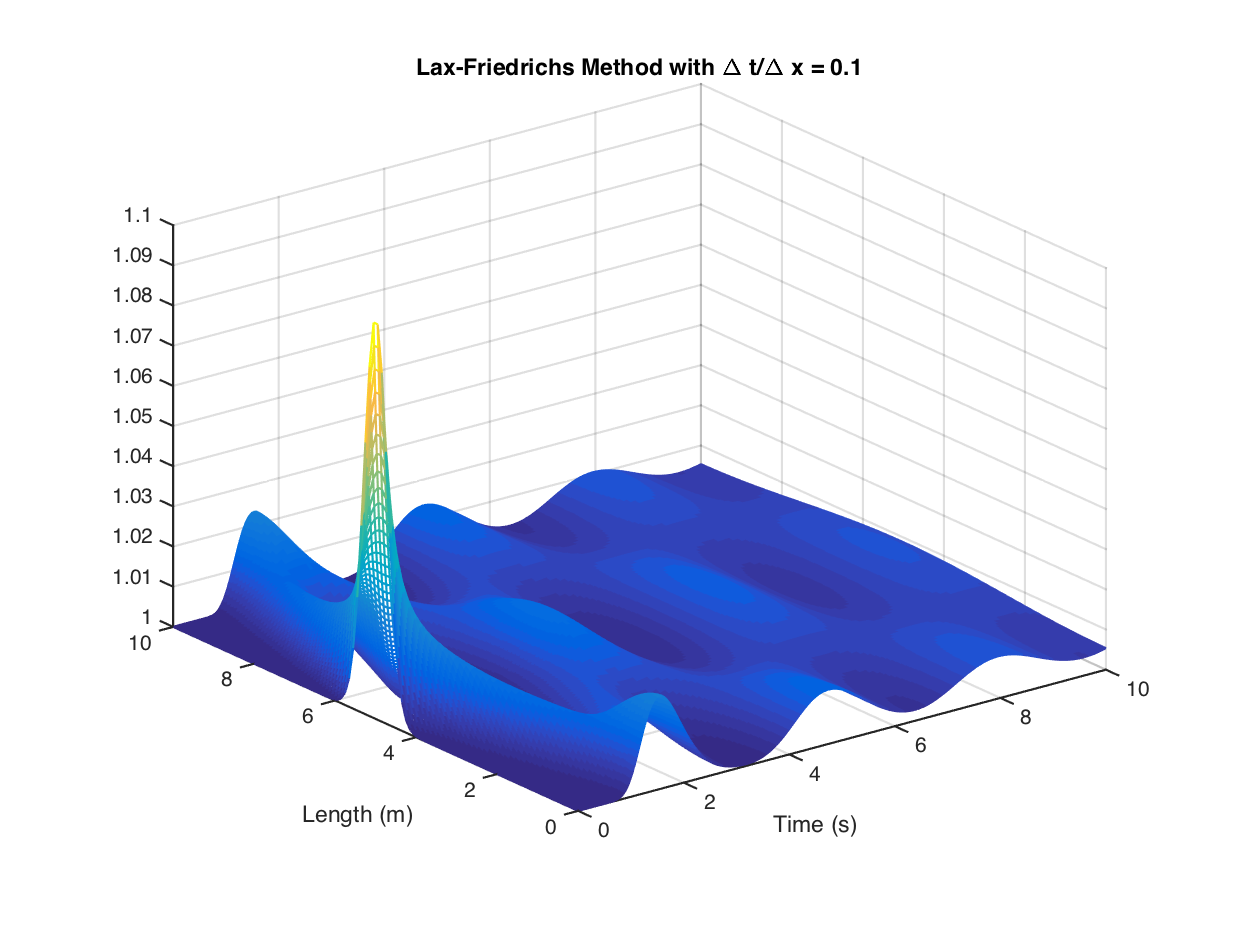
\includegraphics[scale=0.6]{lax01.eps}
\caption{Stable for $\Delta t/\Delta x=0.1$}
\end{center}
\end{figure}

\begin{figure}
\begin{center}
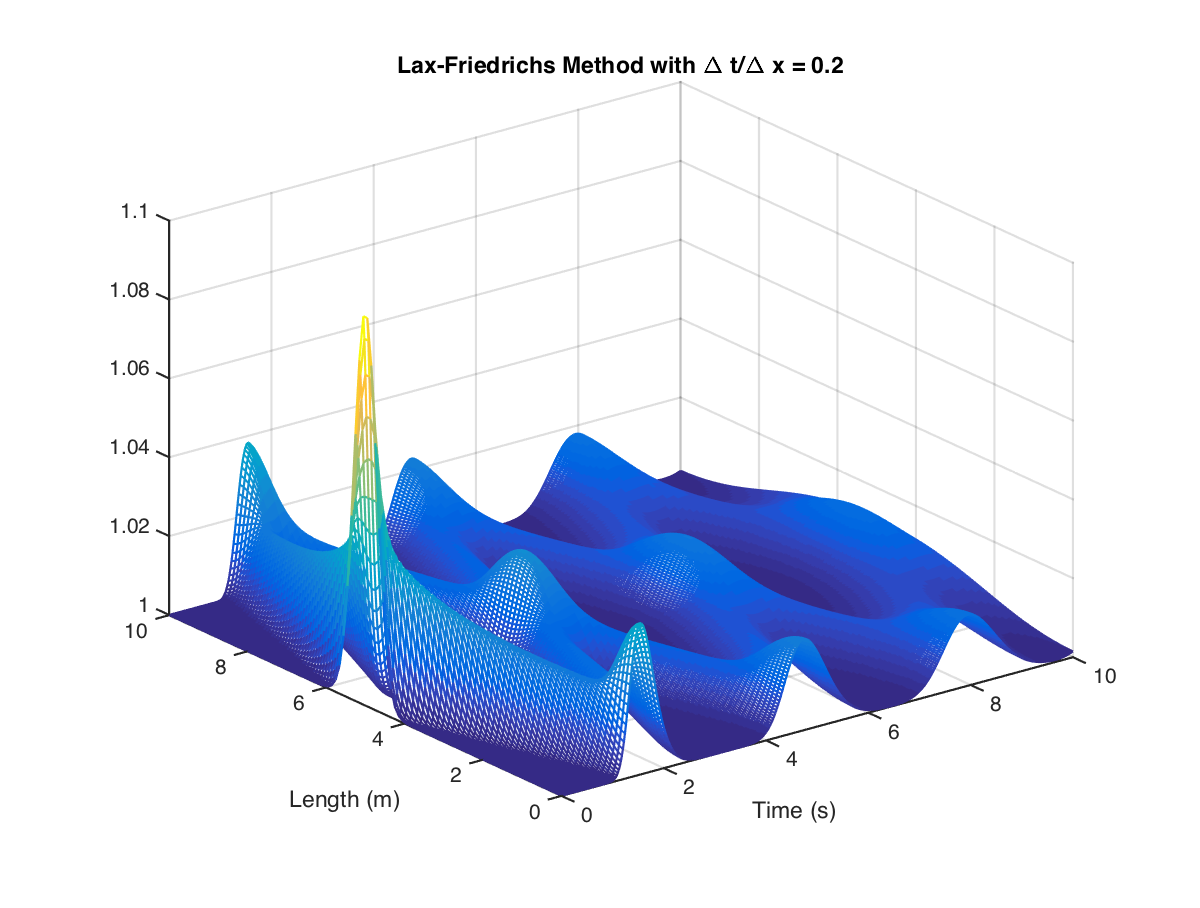
\includegraphics[scale=0.6]{lax02.eps}
\caption{Stable for $\Delta t/\Delta x=0.2$}
\end{center}
\end{figure}

\begin{figure}
\begin{center}
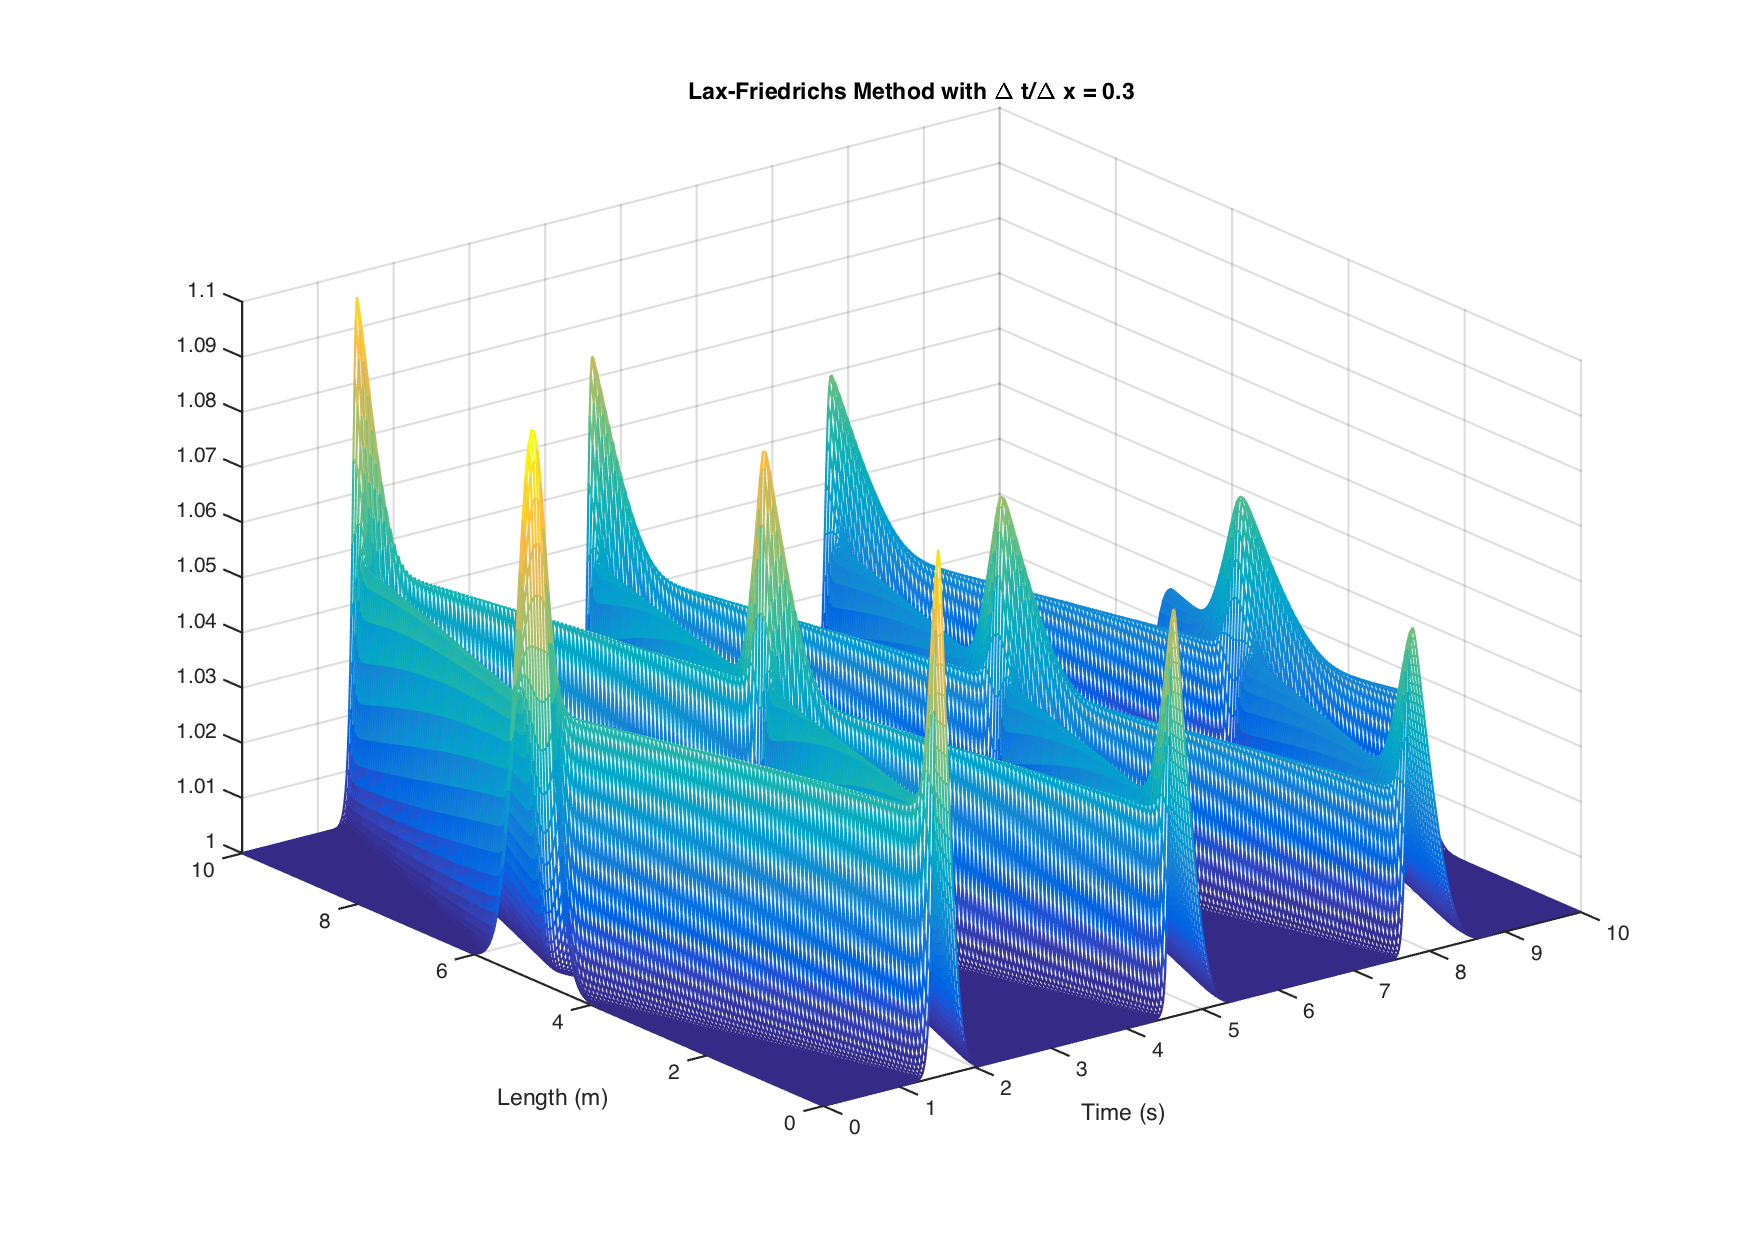
\includegraphics[scale=0.6]{lax03.eps}
\caption{Stable for $\Delta t/ \Delta x=0.306$ and $\Delta x = 200$}
\label{reg}
\end{center}
\end{figure}

\begin{figure}
\begin{center}
\includegraphics[scale=0.6]{lax307.eps}
\caption{Unstable for $\Delta t /\Delta x=0.307$}
\end{center}
\end{figure}

As we can see, in our problem, the Lax-Friedrichs method becomes unstable at $\Delta t/\Delta x=0.307$. The CFL condition is a necessary so we are able to infer that the CFL condition is satisfied up until and including $\Delta t/\Delta = 0.3$. Another thing that is seen is that that the smaller $\Delta t/\Delta x$ is (the larger $\Delta x$ is compared to $\Delta t$), the larger the wave dampening. This also implies that the closer we get the CFL condition, the less wave dampening is observed. 

We are not able to make any comparisons with the values computed in the first part of this assignment because of the different characteristics of the problems investigated. For example, the equation in problem one is a linear parabolic pde, while the equation in this part is a nonliner hyperbolic pde. 

